\begin{enumerate}
	\item $ABCD$ is a cyclic quadrilateral. If $\angle BAD = (2x + 5)^{\circ}$ and $\angle BCD = (x + 10)^{\circ}$ then $x$ is equal to:
		\begin{figure}[h]
			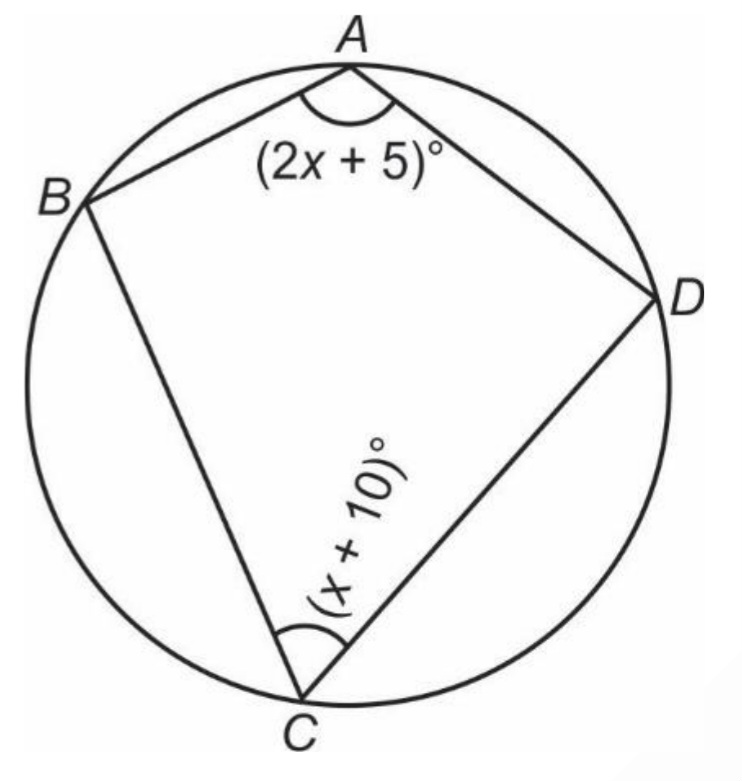
\includegraphics[width=\columnwidth]{figs/img2.jpg}
			\caption{}
			\label{figure}
		\end{figure}
		\begin{enumerate}
			\item $65^{\circ}$
			\item $45^{\circ}$
			\item $55^{\circ}$
			\item $5^{\circ}$
		\end{enumerate}
		\newpage
	\item In the given figure $O$ is the centre of the circle. $PQ$ and $PR$ are tangents and $\angle QPR = 70^{\circ}$. Calculate:
		{\begin{figure}[h]
			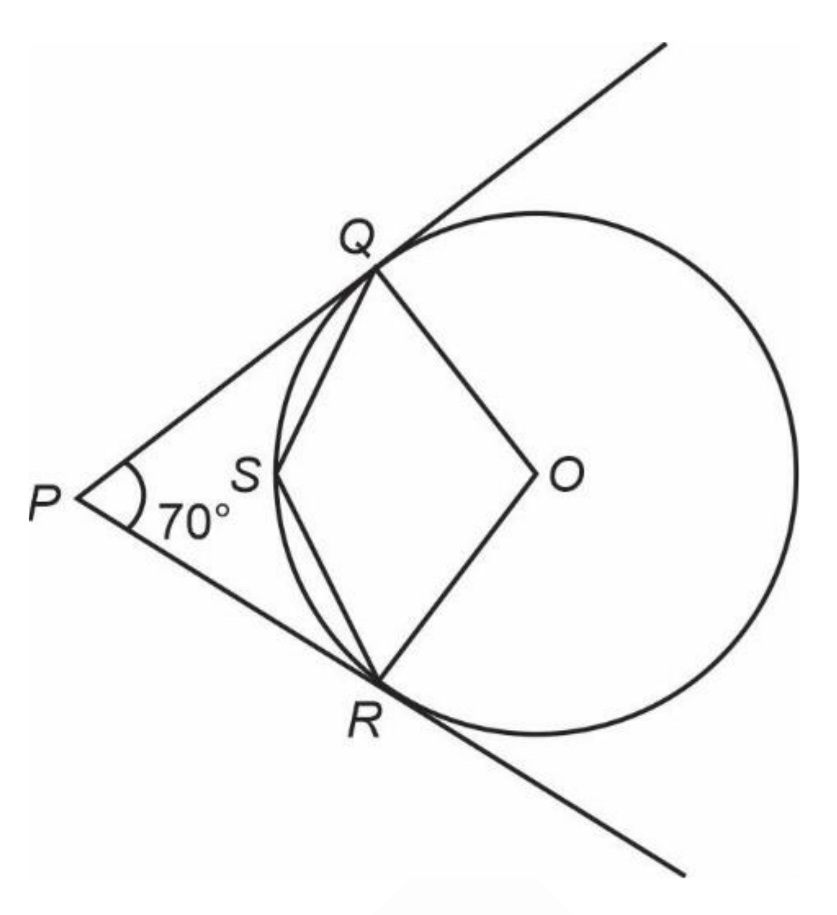
\includegraphics[width=\columnwidth]{figs/img3.jpg}
			\caption{}
			\label{figure}
		\end{figure}}
		\begin{enumerate}
			\item $\angle QOR$
			\item $\angle QSR$
		\end{enumerate}	
	\item Two chords $AB$ and $CD$ of a circle intersect extenally at $E$. if $EC = 2 cm$, $EA = 3 cm$ and $AB = 5 cm$, find the length of $CD$.
		\begin{figure}[h]
			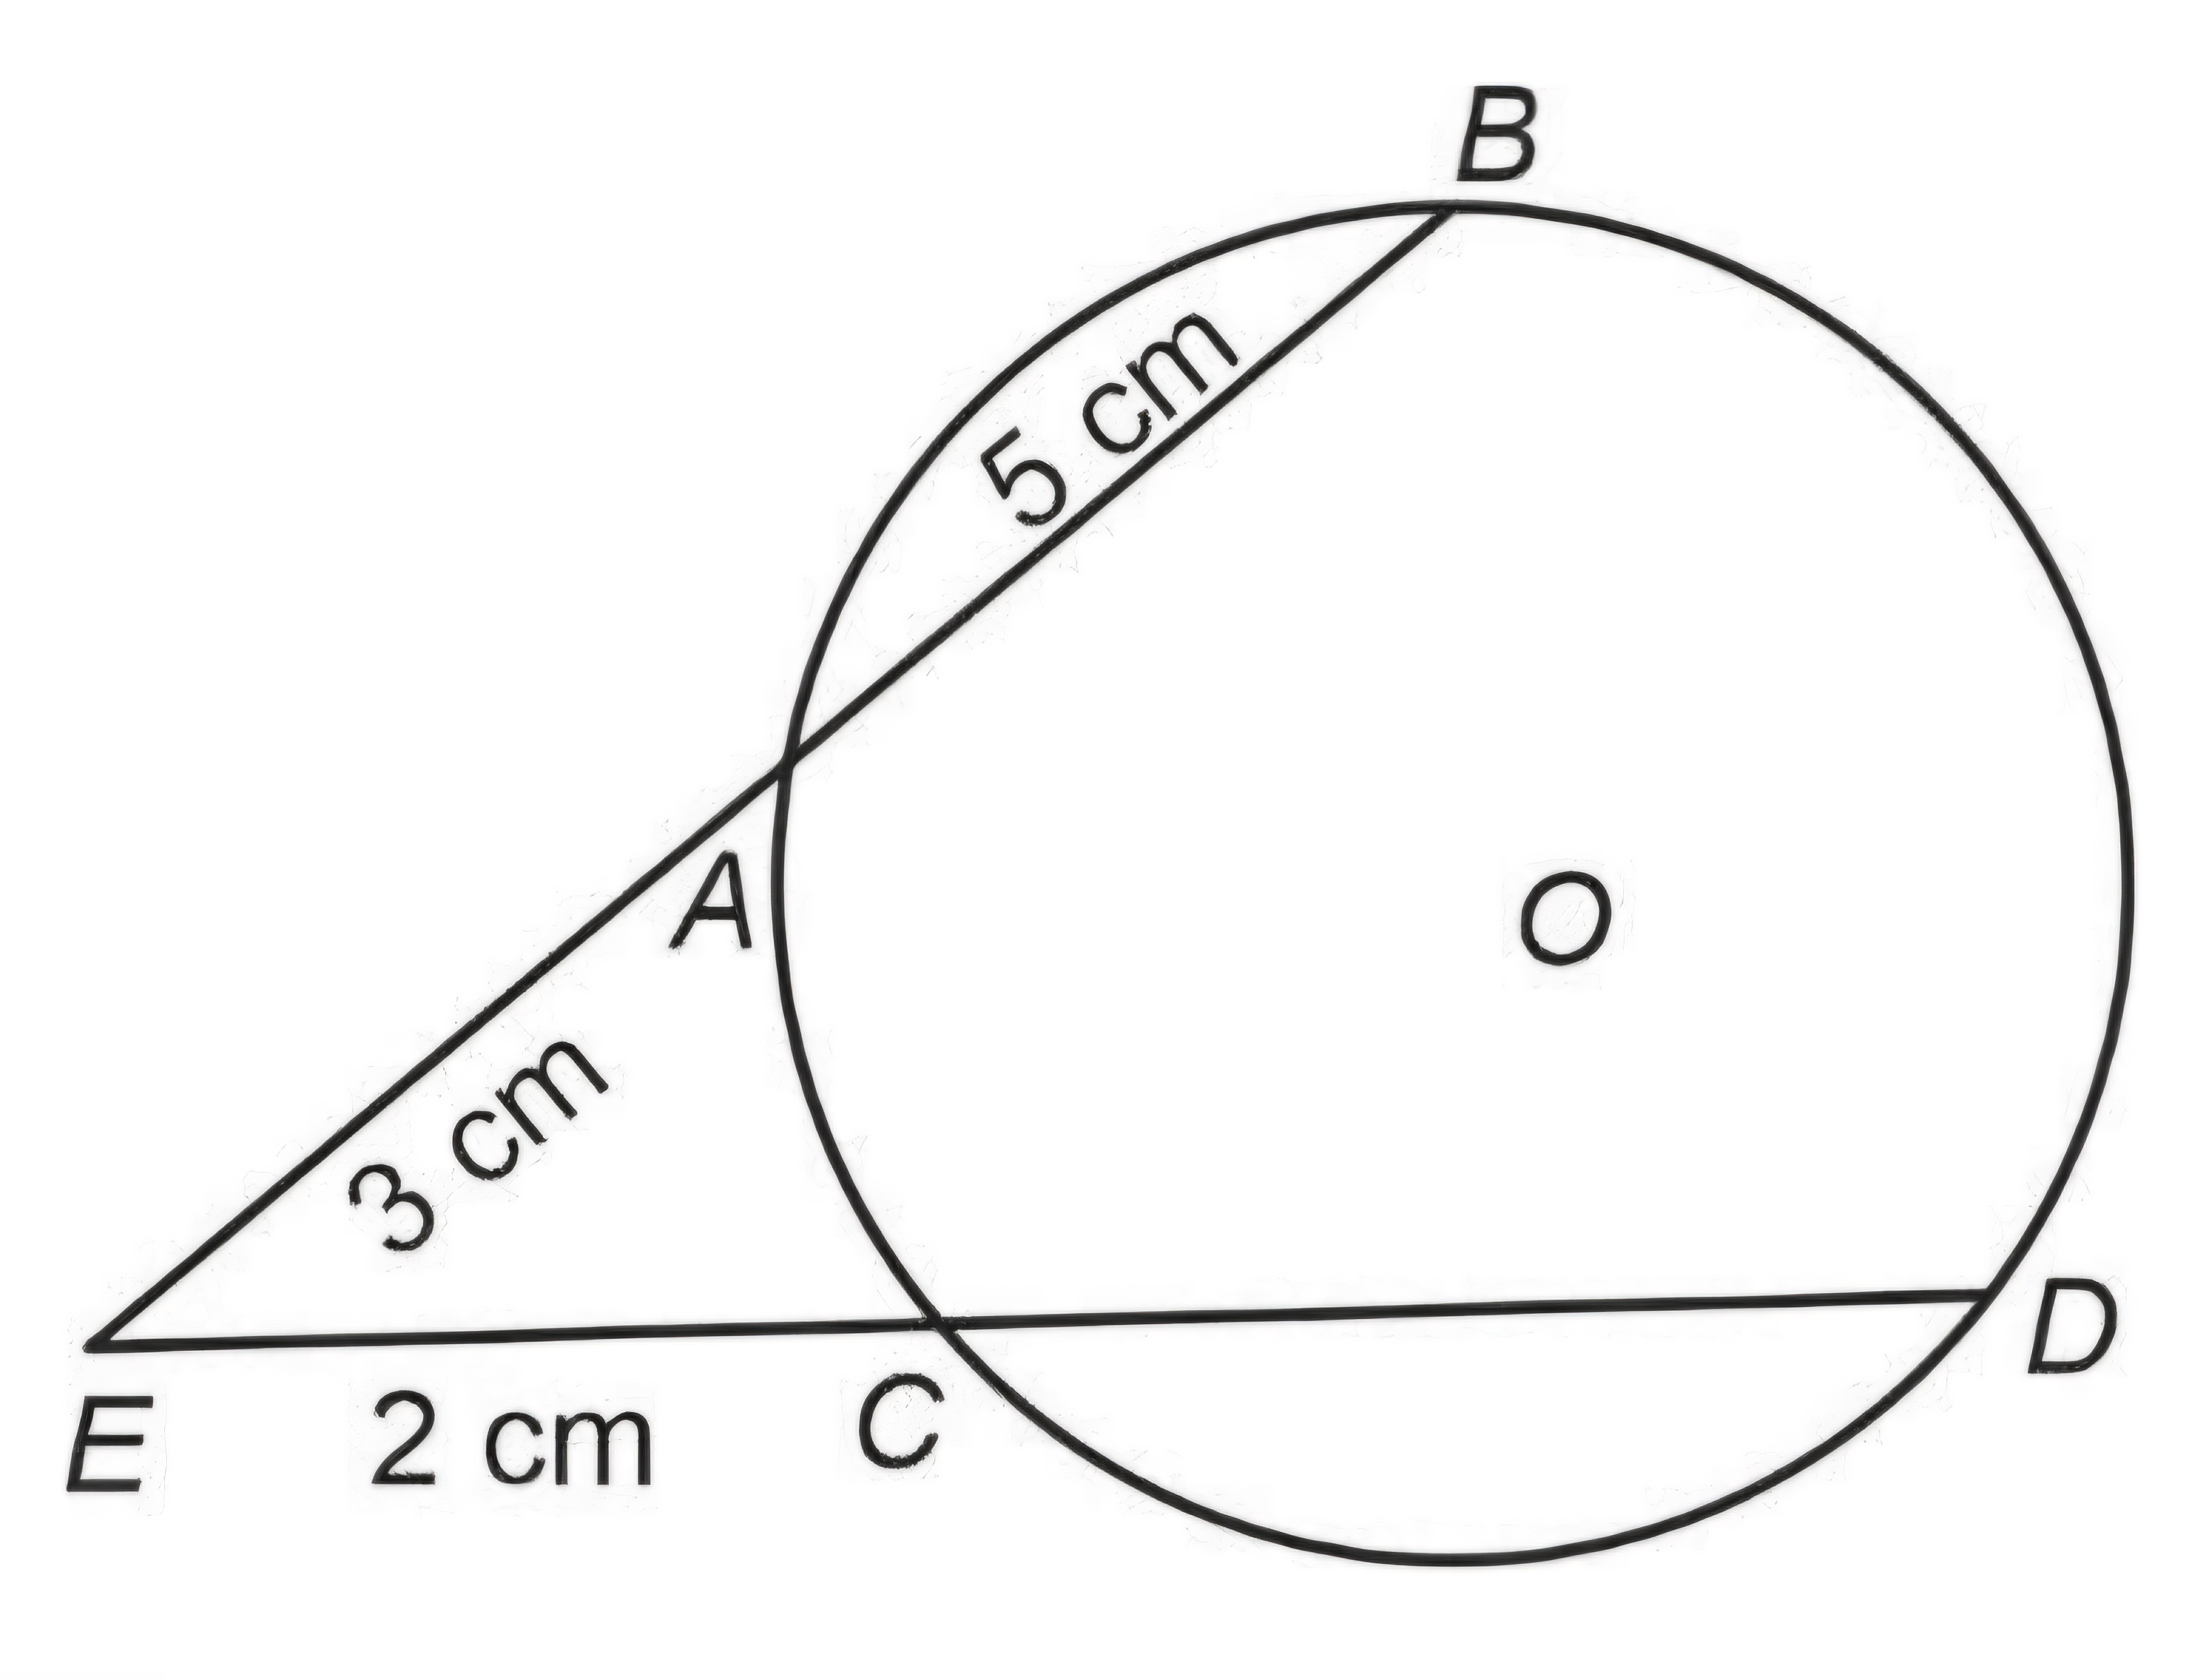
\includegraphics[width=\columnwidth]{figs/img4.jpg}
			\caption{}
			\label{figure}
		\end{figure}
		\newpage
	\item In the given figure $A,B,C$ and $D$ are points on the circle with centre $O$. Given $\angle ABS = 62^{\circ}$. Find:
		\begin{enumerate}
			\item $\angle ADC$
			\item $\angle CAB$
		\end{enumerate}
		\begin{figure}[h]
			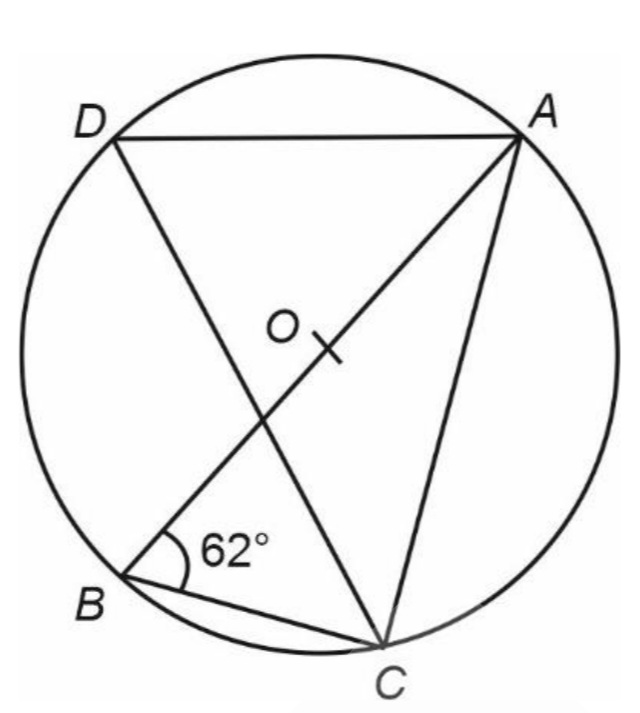
\includegraphics[width=\columnwidth]{figs/img5.jpg}
			\caption{}
			\label{figure}
		\end{figure}
\end{enumerate}  
